\documentclass[a4paper, 11pt]{article}
\usepackage[brazil]{babel}
\usepackage[utf8]{inputenc}
\usepackage{blindtext}
\usepackage[top=3cm, left=2.5cm, right=2cm, bottom=2cm]{geometry}
\usepackage{amsthm,amsfonts}
\usepackage{graphicx}
\graphicspath{ {./img/} }
\setlength\parindent{0pt}

\author{Frederico Queiroz}
\title{Conceitos e Definições - Capítulo 2 Summerville}

\begin{document}
\maketitle

\section{Processo de Software}
\begin{itemize}
	\item \textbf{Processo de Software} é o conjunto de atividades que leva ao desenvolvimento do produto software.
	\item Um processo define:
	\begin{itemize}
        \item \textbf{Quem} faz, \textbf{o que} faz e \textbf{quando} fazer.
        \item Nem sempre diz \underline{como} fazer.
    \end{itemize}
\end{itemize}

\section{Modelo de Processo}
\begin{itemize}
    \item Descrição simplificada do processo.
    \item Definem:
    \begin{itemize}
        \item As atividades para o desenvolvimento do software.
        \item Especificam os produtos de cada atividade.
        \item Indicam os papéis das pessoas envolvidas.
    \end{itemize}
    \item \textbf{Vantagens}:
    \begin{itemize}
        \item Oferecem um roteiro útil para o trabalho de engenharia de software.
        \item Padronização dos artefatos.
        \item Melhor comunicação da equipe.
        \item Menos treinamento de pessoal.
    \end{itemize}
\end{itemize}

\subsection{Exemplos de Modelos de Processo}
\begin{itemize}
    \item Modelos de processo mais gerais:
    \begin{itemize}
        \item Modelo Cascata.
        \item Desenvolvimento Incremental.
        \item Eng. de Software orientada a Reuso.
    \end{itemize}
    \item Modelos que lidam com mudanças:
    \begin{itemize}
        \item Prototipagem.
        \item Entrega Incremental.
        \item Modelo Espiral.
    \end{itemize} 
    \item Os modelos de processos não são mutuamente exclusivos.
    \item Organizações tendem a combinar partes de diferentes modelos em seus processos.
    \item Qual modelo de processo usar?
    \begin{itemize}
        \item \textbf{Sistemas Críticos}: Modelo de processo mais estruturado e rigoroso (Ex.: Modelo Cascata).
        \item \textbf{Sistemas de Negócios (requisitos mudam com frequencia)}: Modelo de processo ágil e flexível (Ex.: Desenvolvimento Incremental, Baseado em Reuso).
    \end{itemize} 
\end{itemize}

\section{Modelo Cascata}
\begin{itemize}
    \item Atividades são sequenciais.
    \item Uma fase deve ser terminada para a outra começar (raramente ocorre na prática).    
\end{itemize}

\begin{figure}[h]
    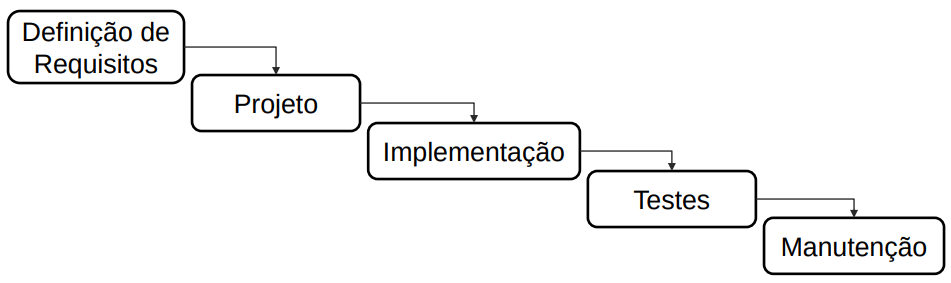
\includegraphics[width=14cm]{modelo_cascata}
    \centering
\end{figure}

\subsection{Vantagens do Modelo Cascata}
\begin{itemize}
    \item Documentação rígida (idealmente completa) em cada atividade.
    \item Reflete abordagens adotadas em outras engenharias.
    \item Aderência a outros modelos de processo (Pode ser combinado a outros modelos).
\end{itemize}

\subsection{Desvantagens do Modelo Cascata}
\begin{itemize}
    \item Projetos reais raramente seguem um fluxo sequencial.
    \item Em geral, é difícil para o cliente estabelecer todos os requisitos à priori.
    \item Difícil se adequar a mudanças inevitáveis de requisitos.
    \item Uma versão executável somente ficará pronta na fase final do projeto.
\end{itemize}

\subsection{Quando Aplicar o Modelo Cascata?}
\begin{itemize}
    \item Sistemas críticos.
    \item Quando os requisitos são bem compreendidos.
    \item Quando há pouca probabilidade dos requisitos mudarem.
\end{itemize}
\newpage

\section{Desenvolvimento Incremental}
\begin{itemize}
    \item Atividades são intercaladas.
    \item \textbf{Objetivo}: dar feedback rápido ao cliente
\end{itemize}

\subsection{Vantagens do Modelo Desenvolvimento Incremental}
\begin{itemize}
    \item Custo de acomodar mudanças nos requisitos é reduzido.
    \item Mais fácil obter feedback do cliente.
    \item Permite trabalhar com o cliente o entendimento dos requisitos.
    \item Pode-se começar o sistema pelas partes melhor entendidas.
\end{itemize}

\subsection{Desvantagens do Modelo Desenvolvimento Incremental}
\begin{itemize}
    \item O processo pode não ser muito claro.
    \item A gerência do software é complicada (O sistema não é completamente especificado à priori).
    \item A estrutura do produto tende a se corromper com a adição de incrementos (O produto final pode se tornar mal estruturado).
    \item \textbf{Obs}: Os problemas do desenvolvimento incremental se tornam mais graves em sistemas críticos.
\end{itemize}

\begin{figure}[h]
    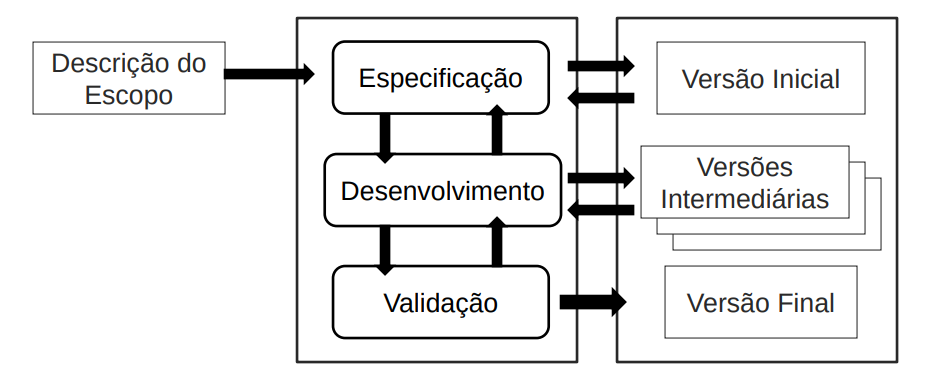
\includegraphics[width=14cm]{modelo_desenv_incremental}
    \centering
\end{figure}
\newpage


\section{Engenharia de Software Orientada ao Reuso}
\begin{itemize}
    \item Baseia-se na existência de um número significativo de componentes reusáveis.
    \item O processo se concentra na integração dos componentes reusáveis.
    \item Inspirado na analogia com componentes (módulos) de hardware.
\end{itemize}

\begin{figure}[h]
    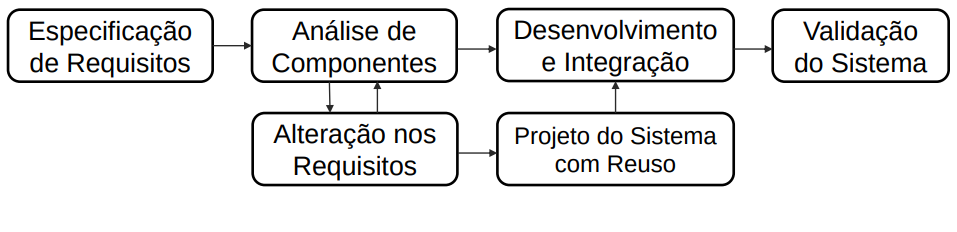
\includegraphics[width=14cm]{modelo_orientado_reuso}
    \centering
\end{figure}

\subsection{Vantagens do Modelo de Eng. de Software Orientada ao Reuso}
\begin{itemize}
    \item Reduz a quantidade de software a ser desenvolvido.
    \item Espera-se reduzir os custos e os riscos.
    \item Espera-se uma entrega do produto mais rápida ao cliente.
\end{itemize}

\subsection{Desvantagens do Modelo de Eng. de Software Orientada ao Reuso}
\begin{itemize}
    \item Pode-se desenvolver um produto que não atenda aos requisitos do cliente.
    \item Pode ser mais difícil evoluir os sistemas (Componentes de terceiros).
    \item A gerência de versões dos componentes pode ser complexa.
\end{itemize}
\newpage

Processos que Lidam com Mudanças:

\section{Prototipação}
\begin{itemize}
    \item Planeja e modela rapidamente um protótipo.
    \item Mais comum na definição de interfaces com os usuários (telas).
    \item É geralmente usada junto com outro modelo de processo.
    \item Objetivo: entender melhor os requisitos.
    \item O protótipo deve ser descartado e o sistema re-implementado usando outro modelo.
    \item \textbf{Principal Vantagem}:
    \begin{itemize}
        \item Auxilia o engenheiro de software e o cliente a entenderem melhor o que deve ser construído.
    \end{itemize} 
\end{itemize}

\section{Entrega Incrementa}
\begin{itemize}
    \item Combina elementos do modelo cascata aplicados de maneira iterativa.
\end{itemize}

\begin{figure}[h]
    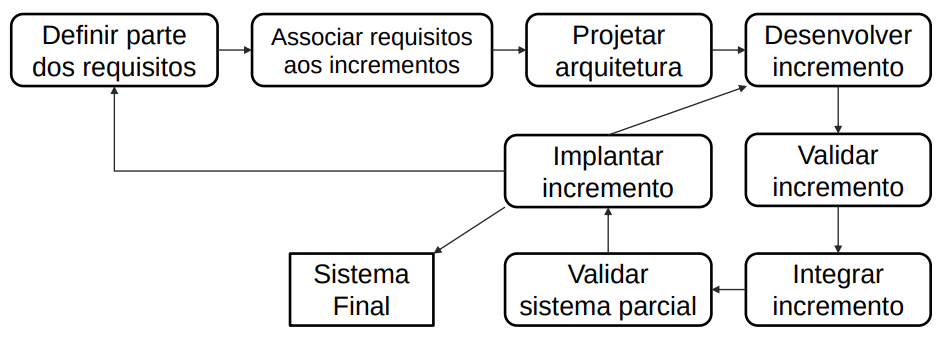
\includegraphics[width=14cm]{modelo_entrega_incremental}
    \centering
\end{figure}

\subsection{Vantagens do Modelo Entrega Incrementa}
\begin{itemize}
    \item Os clientes não precisam esperar a entrega final do sistema. Podem usar o sistema parcial.
    \item Serviços de mais alta prioridade podem ser entregues primeiro.
    \item O risco de falha global do projeto é menor que o Modelo Cascata.
\end{itemize}

\subsection{Desvantagens do Modelo Entrega Incrementa}
\begin{itemize}
    \item Pode ser difícil definir os recursos comuns e propriedades globais dos sistema.
    \item Difícil adoção pelos usuários quando um novo sistema (parcial) irá substituir um sistema antigo (completo).
    \item Pode causar dificuldades no fechamento do contrato.
\end{itemize}


\section{Modelo Espiral}
\begin{itemize}
    \item Combina elementos dos \textbf{modelos incrementais} e de \textbf{Prototipagem} (E sequência adotada do Modelo Cascata).
    \item Software é desenvolvido em versões.
    \begin{itemize}
        \item Prototipagem nas primeiras versões.
        \item Incremental nas últimas versões.
    \end{itemize}
\end{itemize}

\begin{figure}[h]
    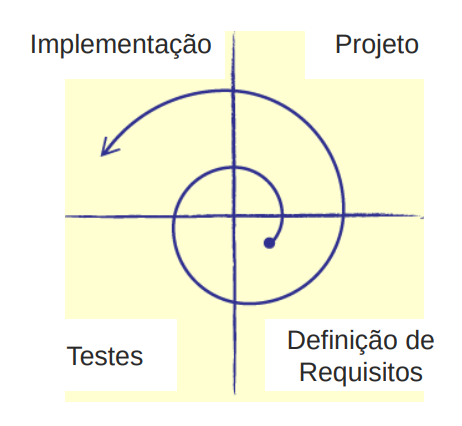
\includegraphics[width=8cm]{modelo_espiral}
    \centering
\end{figure}

\end{document}